% Faz com que o ínicio do capítulo sempre seja uma página ímpar
\cleardoublepage

% Inclui o cabeçalho definido no meta.tex
\pagestyle{fancy}

% Números das páginas em arábicos
\pagenumbering{arabic}

\chapter{Introdução}\label{intro}


\section{Motivação}\label{intro:historico}

\begin{refsection}

Esta tese surgiu da vontade de entender como os processos internos ao
organismo que produzem a variação em uma população interagem com os processos
evolutivos para dar origem à diversidade que observamos na natureza.
Resumidamente, nós procuramos estudar como a covariação genética se estabelece
e como ela evolui, e situamos essas questões dentro do contexto da
macroevolução de caracteres quantitativos. Para isso, nos valemos da teoria de
genética quantitativa na sua encarnação mais moderna, aliada a teoria de
evolução e das técnicas de mapeamento de loci de caracteres quantitativos.
Essa combinação permite estudar e prever as consequências das restrições
genéticas na evolução dos caracteres, e esmiuçar a arquitura genética por traz
dessas restrições. Nesta introdução, vamos revisar rapidamente a teoria de
genética quantitativa evolutiva e discutir a estrutura geral da tese. Neste
capítulo vamos utilizar as citações de forma esparsa, de forma a deixar o texto mais
fluido. A maior parte do contexto teórico pode ser encontrado em livros
básicos de evolução e genética, como~\textcite{Falconer1996-ot,
Lynch1998-ql, Barton2007-hq}. Alguns trechos mais avançados podem ser
encontrados em~\textcite{Rice2004-jf, Buerger2000-ez}. Argumentos que surgiram
em artigos específicos e são mais associados a essa referencia serão
apontados no texto.

\section{Variação genética e evolução} 

A variação fenotípica presente em uma população é fundamental para que a
evolução natural possa ocorrer. Em última instância, a variação fenotípica que
está disponível para que a evolução aconteça é consequência da variação
genética da população\footnote{A rigor variação genética não é estritamente
necessária, apenas variação \textit{herdável}. A herança cultural, por exemplo, pode
ser estudada com as ferramentas da evolução. Apesar disso, em populações
naturais, a maior parte da variação herdável é genética}. Essa variação
genética se dá no nível do DNA, com variantes discretas que segregam na
população. A informação genética contida nessas variantes é interpretada pelo
processo de desenvolvimento, e por meio de um sistema impossivelmente
complicado de interações, a cada geração um novo individuo é formado a partir
da informação no código genético. Mendel descreveu as leis que regem a herança
dessas variantes discretas estudando caracteres de herança discreta e simples,
ervilhas verdes ou amarelas, lisas ou rugosas. Mesmo esses caracteres simples,
cuja variação é determinada por um único locus do genoma, tem pro traz de si
um intrincado processo de desenvolvimento. Se para entender a evolução de
qualquer caráter, quanto mais caracteres complexos, fosse necessário um modelo
do processo que leva à sua formação, o estudo de evolução seria um iniciativa
que inviável. Felizmente, essa compreensão total do organismo não é
necessária. Para o estudo de evolução, basta um modelo de como os organismos
mudam. Somente a ligação entre variação genética e mudança fenotípica importa,
não o mecanismo por traz da formação do fenótipo. Se um gene está envolvido no
desenvolvimento de um caráter mas não apresenta variação genética, esse gene
não é importante para entender a evolução do caráter.

\subsection{Genética quantitativa} 

A grande maioria dos caracteres interessantes do ponto de vista evolutivo tem
uma base genética complexa. Tamanho corporal, sucesso reprodutivo, coloração,
forma, são todos caracteres cuja variação é determinada por muitos genes. Por
um lado, isso torna entender a arquitetura genética da variação desses
caracteres uma tarefa complicada, por outro lado, essa base complexa garante
que esses caracteres irão apresentar um padrão de variação contínuo, e
portanto pode ser estudados utilizando as ferramentas da genética
quantitativa. A variação continua que encontramos em caracteres complexos se
deve a dois fatores: a base poligênica e a variação ambiental a que os
fenótipos estão sujeitos. Quando vários genes estão envolvidos na determinação
de um caráter, a junção dos efeitos de herança particulada de cada umas das
variantes em cada um dos locus acaba por definir tantas classes de fenótipos
que a variação pode ser tratada como contínua. Além disso, se assumirmos que
cada gene contribui de forma aditiva ao fenótipo, o teorema do limite central
diz que a distribuição do caráter na população pode ser aproximado por uma
distribuição gaussiana. Na prática, a grande maioria dos caracteres de
interesse evolutivo podem ser aproximados por uma distribuição
normal\footnote{Interessantemente, a observação de que a distribuição
Gaussiana era tão ubíqua e útil na biologia evolutiva foi feita inicialmente
por um primo de Darwin, Francis Galton, em 1969}, ou transformados
trivialmente para uma distribuição normal\footnote{Caracteres contínuos que
são restritos a valores positivos, como distancias ou pesos, podem apresentar
uma distribuição log normal, em que o log das medidas tem distribuição normal.
Essa transformação implica que os genes tem efeitos multiplicativos no
fenótipo, e a transformação log transforma essas multiplicações em adições,
levando à distribuição normal após a transformação.}. Além disso, existe
diferenças ambientais no desenvolvimento de um caráter. Mesmo uma população de
indivíduos geneticamente idênticos irá apresentar alguma variação em seus
caracteres. Essa variação ambiental contribui para o aumento do número de
fenótipos possíveis e para a possibilidade de descrever a variação como
contínua (Fig.~\ref{discrete_aleles}).

\begin{figure}
    \centering
    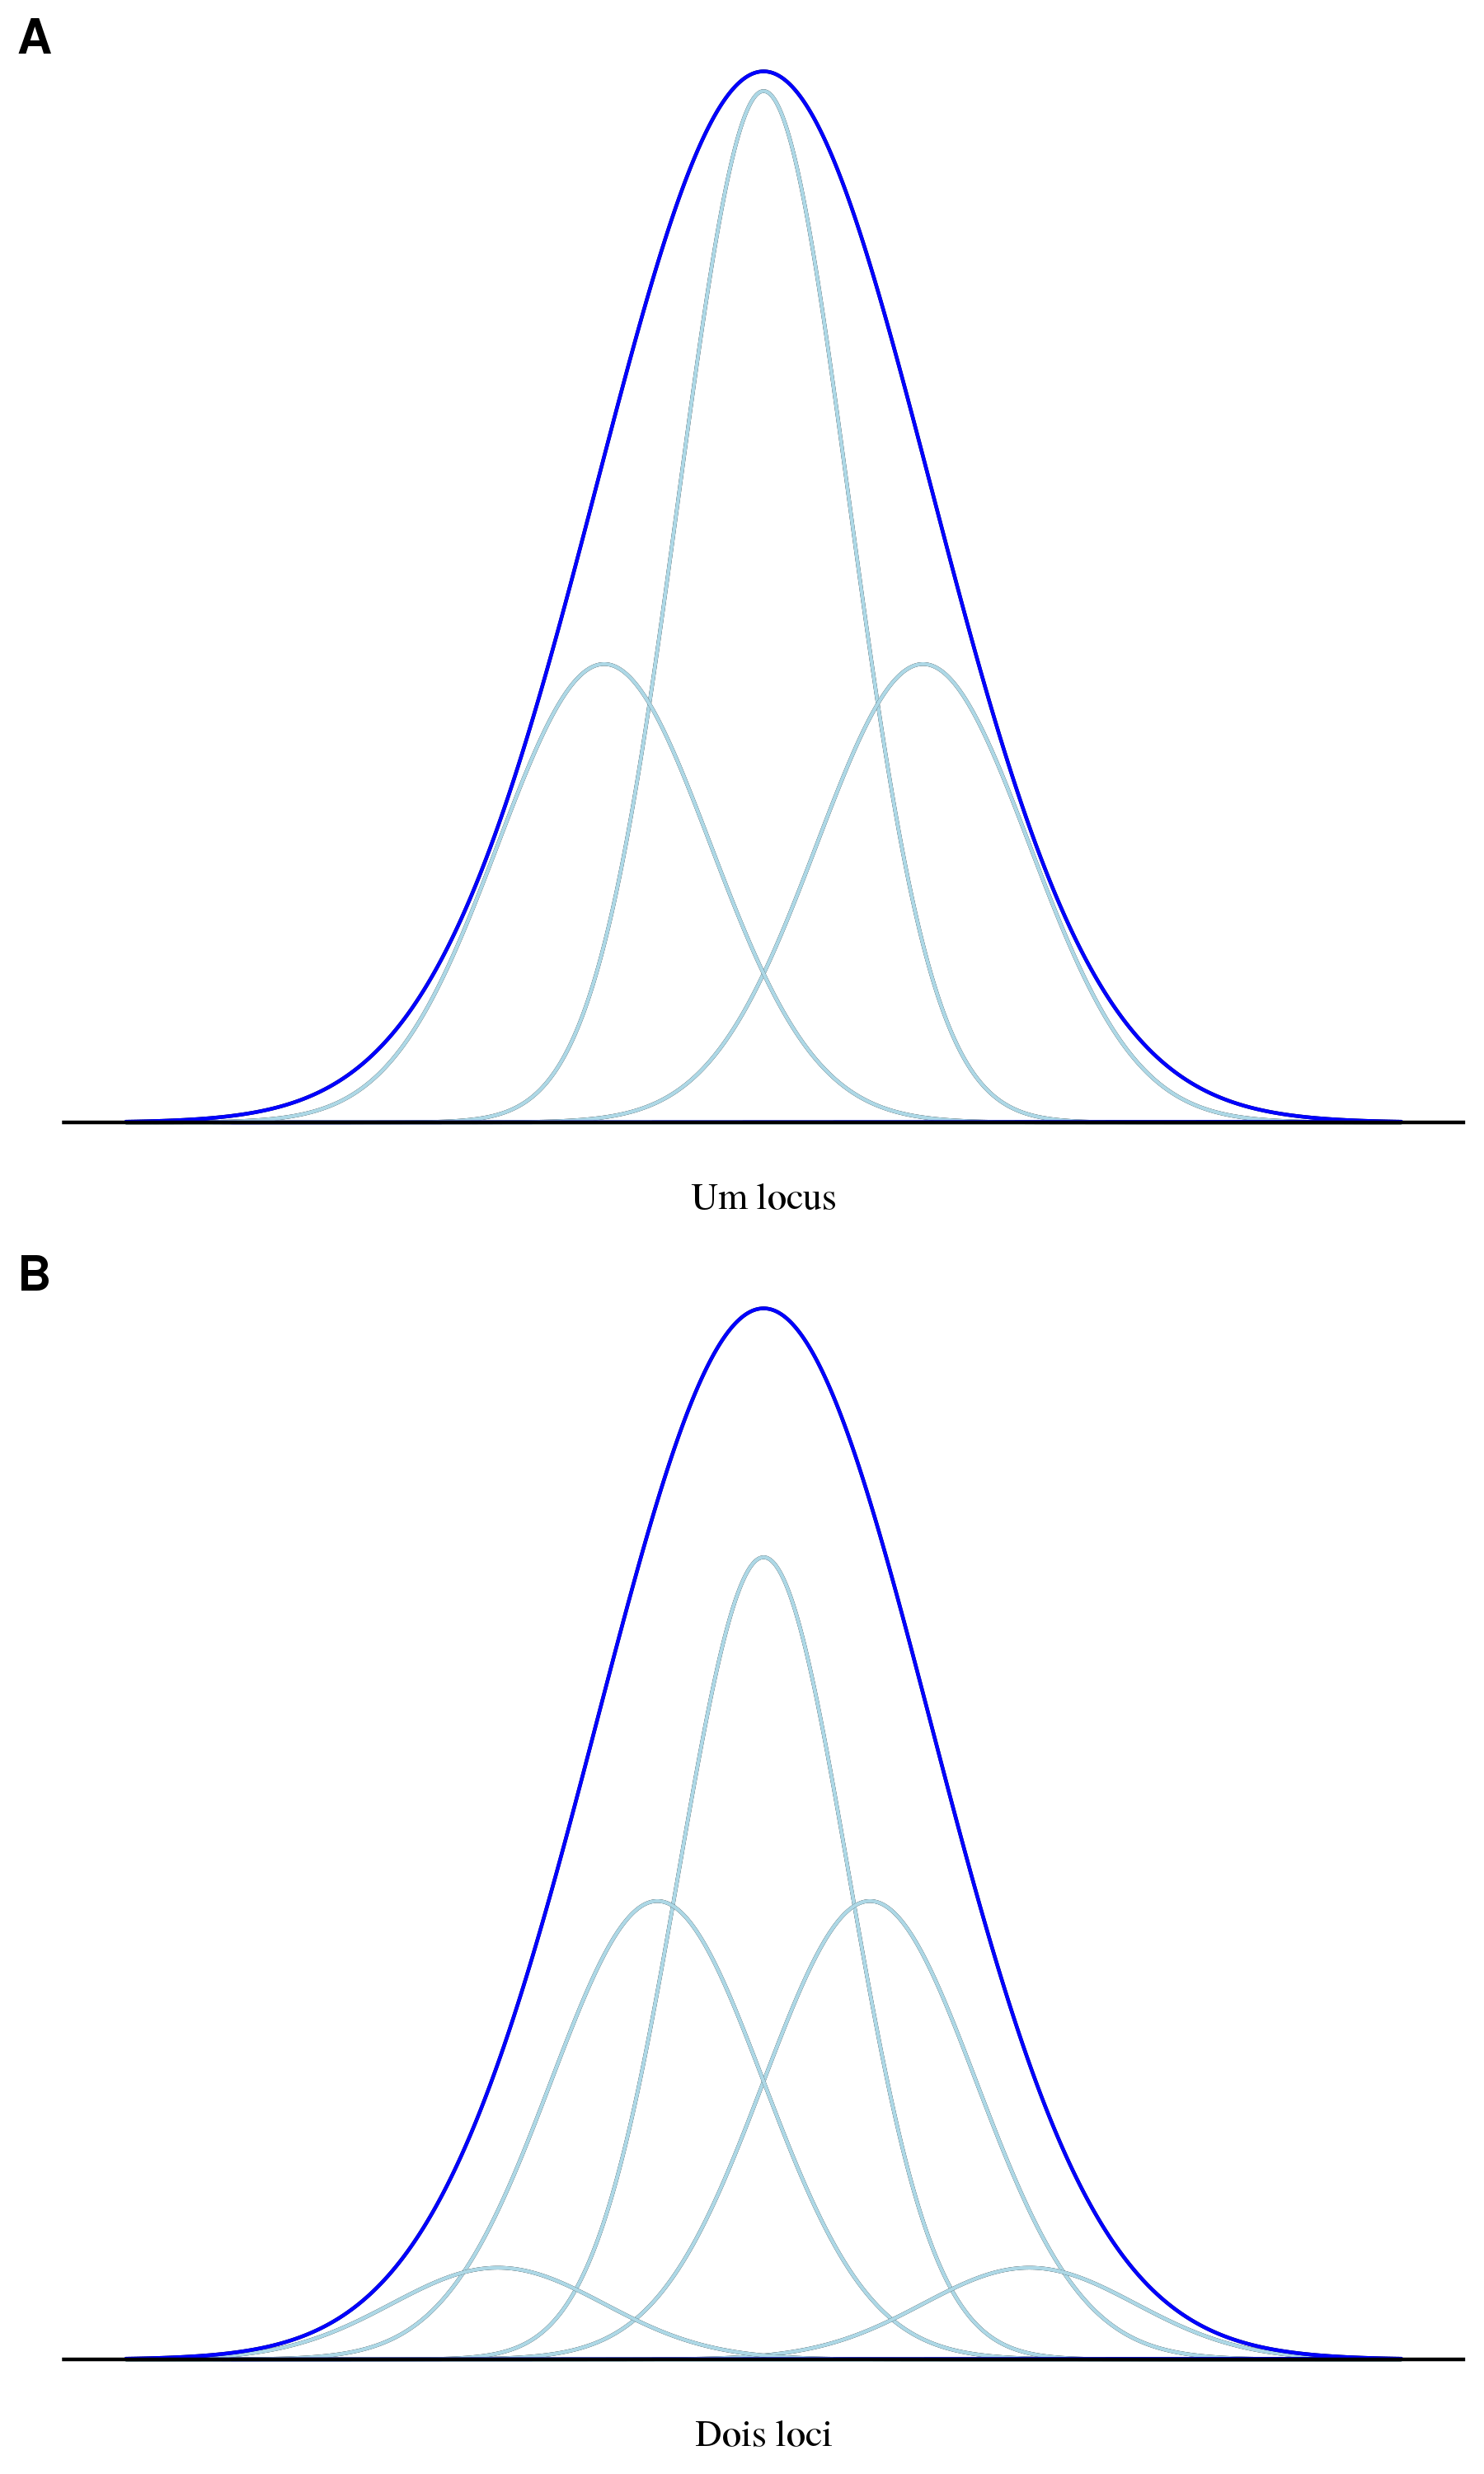
\includegraphics[width=300px]{discrete_gaussian.png}
    \caption[Variação contínua]{Mesmo com poucos loci, o modelo aditivo e variação ambiental são capazes de gerar distribuições fenotípicas muito próximas à gaussiana, dado que a diferença entre classes genotípicas seja da mesma escala da variação dentro de cada classe. A) Um loci aditivo com dois alelos de mesma frequência e a variação ambiental dentro de cada genótipo. As linhas finas mostram a variação dentro de cada classe, e a linha grossa a distribuição na população. B) Dois loci com dois alelos cada, com efeitos fenotípicos equivalentes. Adaptado de~\textcite{Barton2007-hq}.}
    \label{discrete_aleles}
\end{figure}

A ideia que a variação de um fenótipo pode ser expressa como a soma de vários
efeitos aditivos independentes, proposta por~\textcite{Fisher1930-bp}, é
central para a genética quantitativa. A primeira distinção é entre os
componentes devido a diferenças genéticas entre os indivíduos e o componente
devido a diferenças não genéticas (ambientais) da variação em uma população.
Para entender como o fenótipo é composto, podemos definir $G$ como a média do
fenótipo dos indivíduos que tem um determinado genótipo e $E$ como o desvio
devido ao ambiente. O fenótipo $P$ do indivíduo então é definido como:

\begin{equation}
P = G + E
\end{equation}

Como $G$ é definido como a média de $P$, a média de $E$ deve ser zero. Se a
distribuição de efeito ambientais for aproximadamente normal e se não existe
interação entre $E$ e $G$, ou seja, se a variação ambiental for a mesma para
todos os genótipos, um genótipo pode ser descrito apenas pelo seu valor
genotípico $G$ e pela sua variância ambiental $V_E$. Se a população em questão
é formada de indivíduos sexuados, o valor genotípico de um indivíduo será
composto pelas contribuições dos gametas parentais. Suponha que para os dois
locus que afetam um dado caráter o indivíduo tenha recebido um gameta $A_1B_1$
do pai e um gameta $A_2B_1$ da mãe. Então, o genótipo do indivíduo é
$A_1A_2B_1B_1$, heterozigoto no locus A e homozigoto no locus B. Dentro de um
modelo aditivo, no qual os efeitos de cada alelo são somados, o fenótipo do
indivíduo seria $P = \alpha_{A_1} + \alpha_{A_2} + 2\alpha_{B_1}$ + E, onde os
$\alpha$ representam as contribuições aditivas de cada alelo, que junto
compõem o valor genotípico do indivíduo. 

Naturalmente, o modelo puramente aditivo é uma simplificação enorme, e, na
prática, existem dois tipos de interações importantes entre alelos que podem
contribuir com o valor genotípico: interações de dominância, que acontecem
entre alelos do mesmo locus, e interações epistáticas, que acontecem entre
alelos em locus diferentes. Dominância acontece quando os efeitos dos alelos
em um locus não são simplesmente aditivos, ou, em outras palavras, quando o
heterozigoto não tem valor genotípico intermediário aos dois homozigotos
correspondentes. Já epistasia acontece quando o efeito de um alelo em um locus
depende do estado de outro locus. Ambas formas de interação são extremamente
comuns e contribuem de forma decisiva para mudança evolutiva, principalmente
epistasia, como veremos mais adiante.

Dentro do formalismo da genética quantitativa, as interações entre alelos e locus podem ser incluídas na formação do valor genotípico, também de forma aditiva. Então, a equação para o fenótipo de um indivíduo se torna:

\begin{equation}
P = G + E = A +D + I + E
\end{equation}

na qual nós decompomos o valor genotípico na sua porção devido aos efeitos
aditivos ($A$), de dominância ($D$) e epistáticos ($I$, interação). O termo
$A$ também é chamado de valor de acasalamento, e, além de ser a soma das
contribuições aditivas de cada alelo, este termo tem uma interpretação simples
que não faz referencia à base genética do fenótipo. O valor de acasalamento de
um indivíduo para um fenótipo pode ser definido como duas vezes a diferença
entre a média do fenótipo da sua prole com parceiros escolhidos ao acaso na
população e a média do fenótipo da população como um todo. A diferença é
dobrada pois o individuo contribui com metade do valor genotípico dos seus
filhos, a outra metade vindo ao acaso da população.

\subsubsection{Componentes da variação fenotípica}

Apesar de conceitualmente importantes, são raras as ocasiões em que temos
condição de medir valores dos componentes genotípicos de um indivíduo. Estimar
esse valores envolveria conhecer o genótipo de todos os indivíduos de uma
população em todos os locus que fossem de alguma forma envolvidos na formação
do fenótipo do indivíduo, uma tarefa praticamente impossível. A importância
prática desse esquema de decomposição fica mais clara quando consideramos a
variação população como um todo. A decomposição da variância da população nos
seus componentes devido a efeitos aditivos, de dominância e todos os outros
componentes do fenótipo pode ser feita sem nenhuma referencia à base genética
específica do fenótipo. Supondo que a variação genética e ambiental são
independentes, podemos expressar a variação fenotípica ($V_P$) como a soma das
variâncias genéticas e ambientais:

\begin{equation}
V_P = V_G + V_E
\end{equation}

Do mesmo modo, a variância dos valores genotípicos pode ser subdividida nos termos devido as diferentes tipos de efeitos genéticos:

\begin{equation}
V_G = V_A + V_D + V_I
\end{equation}

O componente da variância devido a diferenças nos valores de acasalamento
($V_A$) é chamado de variância genética aditiva, e tem um papel fundamental na
biologia evolutiva. O componente devido a interações epistáticas, $V_I$,
também pode ser subdivido em diferentes tipos de interação entre dois loci:
entre componentes aditivos ($V_{AA}$), entre componentes aditivos e de
dominância ($V_AD$), entre componentes de dominância ($V_DD$), e mesmo
componentes de grau mais alto, entre 3 ou mais loci. Essa subdivisão fornece
uma ferramenta poderosa para o estudo da variação e evolução em populações
naturais.

Cada um desses componentes pode ser estimado a partir da semelhança entre
indivíduos relacionado em uma população. Por exemplo, no caso da similaridade
entre pais e filhos, fundamental na herança de caracteres e para a evolução.
No caso mais simples, no modelo aditivo, o fenótipo de um indivíduo é dado por
$P = A + E$, e o componente aditivo pode ser subdividido em duas partes, as
contribuições do pai e da mãe, então $P = A_1 + A_2 + E$. Já o fenótipo do pai
pode ser escrito como $P_F = A_1 + A_3 + E_F$, onde $A_1$ representa a porção
do valor de acasalamento compartilhada com o filho e $A_3$ a porção
independente do filho. A covariação entre pai e filho então é $cov(P, P_F) =
cov(A_1 + A_2 + E, A_1 + A_3 + E_F)$. A covariância da soma de fatores
independentes pode ser escrita como a soma das covariâncias par a par, então
$cov(P, P_F) = cov(A_1, A_1) + cov(A_1, A_3) + cov(A_2, A_1) + \cdots  +
cov(E, E_F)$. Como todos os componentes são independentes por construção, o
único termo que contribui para a covariância entre pais e filhos é $cov(A_1,
A_1) = var(A_1)$. Como a variância aditiva total é a soma das contribuições
paternas e maternas $V_A = var(A_1) + var(A_2)$, e como as contribuições
paternas e maternas são equivalentes, a covariância entre pais e filhos é a
metade da variância aditiva total ($cov(P, P_F) = var(A_1) = \frac{1}{2}V_A$).
A partir de deduções semelhantes, podemos estimar vários dos componentes da
variação genotípica a partir da covariância entre indivíduos relacionados. Por
exemplo, a variância de dominância pode ser estimada comparando a covariância
entre irmãos completos e pais e filhos, pois irmãos podem compartilhar
genótipos, enquanto pais não compartilham genótipos com os filhos. Então, na
presença de dominância, a covariância entre irmãos é maior que a covariância
entre pais e filhos.

\subsubsection{Herdabilidade e a resposta à seleção}

Como a variância aditiva é a principal responsável pela similaridade entre
indivíduos aparentados, em especial pais e filhos, a proporção da variação
fenotípica que é devido a variação aditiva recebe um tratamento especial
dentro da genética quantitativa, recebendo o nome de herdabilidade. A herdabilidade é
definida como a razão da variância aditiva pela variância fenotípica total: 
$h^2 = \frac{V_A}{V_P}$.\footnote{O quadrado faz parte do simbolo, e se refere
ao fato da herdabilidade ser uma razão de variâncias, e portanto numa escala
quadrática.} 

A herdabilidade é especialmente importante para entender a resposta evolutiva,
pois é a ela que determina como uma mudança na média dos pais se traduz numa
mudança evolutiva na média dos filhos. Essa relação é dada pela equação do
criador, que relaciona a mudança em um fenótipo de uma geração para outra
($R$) com a mudança dentro de uma geração devido a um episódio de seleção ($S$):

\begin{equation}
R = h^2S = \frac{V_A}{V_P}S	
\end{equation}

Essa equação revela que a resposta à seleção depende fundamentalmente da
presença de variação aditiva. Sem variação aditiva, sem herdabilidade, não há
como a mudança em resposta à seleção natural acontecer.

\subsubsection{Resposta à seleção multivariada}

Se estamos interessados em fenótipos complexos, compostos de muitos
caracteres, além de quantificar a variância individual de cada um, podemos
também levar em conta a interação entre eles. De forma análoga à variância, a
covariância mede a variação conjunta de dois caracteres. A matriz de
covariância genética aditiva (matriz G) resume a covariância entre os valores de
acasalamento de caracteres diferentes, enquanto a matriz de covariância
fenotípica (matriz P) reune as variância de covariâncias entre os fenótipos da população. 

A partir dessas matrizes, é possível escrever o análogo multivariado da
equação do criador, a equação de resposta multivariada de~\textcite{Lande1979-by}:

\begin{equation}
\Delta \mathbf{\overline z} = GP^{-1}\mathbf{S}
\end{equation}

Nesse caso, tanto a resposta à seleção ($\Delta \mathbf{\overline z}$) quando a
diferença nas médias antes de depois da seleção dentro da geração parental
($\mathbf{S}$) são representados por vetores, com um componente por caráter
sendo analisado.

\subsection{Estrutura da variação}



\printbibliography
\end{refsection}